\documentclass{beamer}
\usepackage[czech]{babel}
\usepackage[utf8]{inputenc}
\usepackage{minted}

\usetheme{boxes}

% \AtBeginSection[]
% {
%    \begin{frame}
%        \frametitle{Přehled}
%        \tableofcontents[currentsection]
%    \end{frame}
% }
% \AtBeginSubsection[]
% {
%    \begin{frame}
%        \frametitle{Přehled}
%        \tableofcontents[currentsection,currentsubsection]
%    \end{frame}
% }

\title{Python testing tools}
\author{Tomáš Ehrlich}
\date{29. srpna. 2013}

\begin{document}
% Title page
\begin{frame}
\titlepage
\end{frame}

\section{Psaní a spouštění testů}
\subsection{assert}

\begin{frame}
\begin{center}
\huge{\PY{k}{assert} statement}
\end{center}
\end{frame}

\begin{frame}[fragile]
\begin{minted}{python}
"""
examples/assert/euler01.py
Project Euler, problem 1

"""
def multiples35(upper_limit):
    # TODO: This is *not* the real answer
    if upper_limit == 10:
        return [3, 5, 6, 9]
    return []

# Check known outputs
assert multiples35(10) == [3, 5, 6, 9]
assert sum(multiples35(10)) == 23

# TODO: Get real answer
print(sum(multiples35(1000)))
\end{minted}
\end{frame}

\begin{frame}
\begin{itemize}[<+->]
\item Jednoduché
\item Bez konfigurace
\item Může být součástí kódu (odstraněno při optimalizaci {\tt -O})
\end{itemize}
\end{frame}

\begin{frame}[fragile]
Jednoduchý type checking:
\begin{minted}[frame=lines]{python}
# redis_collections/base.py

def _create_new(self, data=None, key=None, ...):
    assert not isinstance(data, RedisCollection), \
        "Not atomic. Use '_data()' within ..."

    cls = cls or self.__class__
    ...
\end{minted}
\end{frame}

\subsection{unittest}

\begin{frame}
\begin{center}
\huge{unittest}
\end{center}
\end{frame}

\begin{frame}[fragile]
\begin{minted}{python}
""" examples/unittest/test_crash.py """
import unittest
from factory import Car

class TestCar(unittest.TestCase):
    def setUp(self):
        self.car = Car()
        car.hit_wall(velocity=120)

    # def tearDown(self): pass

    def test_crash(self):
        self.assertTrue(car.is_damaged)

if __name__ == '__main__':
    unittest.main()

\end{minted}
\end{frame}

\begin{frame}[fragile]
\begin{minted}{python}
% python examples/unittest/test_crash.py
.
---------------------------------------
Ran 1 test in 0.000s

OK

\end{minted}
\end{frame}

\begin{frame}[fragile]
\begin{minted}{python}
F
========================================
FAIL: test_crash (__main__.TestCar)
----------------------------------------
Traceback (most recent call last):
  File "examples/unittest/test_crash.py", line 13, ...
    self.assertFalse(self.car.is_damaged)
AssertionError: True is not false

----------------------------------------
Ran 1 test 0.001s

FAILED (failures=1)
\end{minted}
\end{frame}

\begin{frame}
\begin{itemize}[<+->]
\item Součástí standartní knihovny
\item Od verze 2.7/3.2 obsahuje {\tt test discovery}
\item Sada testů (assertEqual, assertIn, ...)
\item Může se využít dědičnost tříd (django db backends)
\end{itemize}
\end{frame}

\begin{frame}[fragile]
\begin{minted}{python}
class TestCar(unittest.TestCase):
    model = Car

    def setUp(self):
        self.car = self.model()
        ...

class TestBlueCar(TestCar):
    model = BlueCar

class TestHovercraft(TestCar):
    model = Hovercraft

    def test_flying(self):
        ...

\end{minted}
\end{frame}

\begin{frame}
\begin{block}{}
    Komplexních sady testů a porovnání (asserts) s podrobným chybovým výstupem
\end{block}
\end{frame}
\subsection{nose}

\begin{frame}
\begin{center}
\huge{nose}
\end{center}
\end{frame}

\begin{frame}[fragile]
\begin{minted}{python}
def setup_func():
    global car
    car = Car()
    car.hit_wall(velocity=120)

@with_setup(setup_func)
def test_crash():
    global car
    assert car.is_damaged == True

\end{minted}
\end{frame}

\begin{frame}
\begin{itemize}[<+->]
\item Jednoduchý zápis
\item Obsahuje (hlavně) {\tt test discovery}
\item Může spouštět i TestCase z unittestu
\end{itemize}
\end{frame}

\begin{frame}
Množství rozšiřujících modulů:
\begin{itemize}[<+->]
\item Logcapture
\item Test coverage
\item Paralelní spouštění testů
\item Výběr testů podle atributů
\item ...
\end{itemize}
\end{frame}

\begin{frame}
\begin{alertblock}{}
      Nose není testovací framework, ale test runner, který spouštění testů usnadňuje a doplňuje.
   \end{alertblock}
\end{frame}

\subsection{py.test}

\begin{frame}
\begin{center}
\huge{py.test}
\end{center}
\end{frame}

\begin{frame}[fragile]
\begin{minted}{python}
def multiples35(upper_limit):
    # TODO: This is *not* the real answer
    if upper_limit == 10:
        return [3, 5, 6, 9]
    return []

def test_known_inputs():
    # Check known outputs
    assert multiples35(10) == [3, 5, 6, 9]
    assert sum(multiples35(10)) == 23

def test_solution():
    assert sum(multiples35(1000)) != 0
\end{minted}
\end{frame}

\begin{frame}[fragile]
\begin{minted}{text}
% py.test euler01.py
== test session starts ==
platform linux2 -- Python 3.2.3 -- pytest-2.3.5
collected 2 items 

euler01.py .F

== FAILURES ==
__ test_solution __

    def test_solution():
>       assert sum(multiples35(1000)) != 0
E       assert 0 != 0
E        +  where 0 = sum([])
E        +    where [] = multiples35(1000)

euler01.py:20: AssertionError
== 1 failed, 1 passed in 0.05 seconds ==

\end{minted}
\end{frame}

\begin{frame}
\begin{itemize}[<+->]
\item Jednoduchý zápis
\item Podrobnější chybový výstup než nose/assert statement
\item Testy můžou být seskupeny do tříd
\end{itemize}
\end{frame}

\begin{frame}
\begin{block}{}
    Jednoduchost {\tt assert statementu} doplněná o podrobnější chybový výstup jako od {\tt unittestu}.
\end{block}
\end{frame}
\subsection{Srovnání}

\begin{frame}
\begin{center}
\huge{unittest vs. nose vs. py.test}
\end{center}
\end{frame}

\begin{frame}
\begin{itemize}[<+->]
\item unittest má testovací třídy (TestCase s assert*)
\item nose má pluginy (coverage, multiprocessing)
\item py.test má skvělý chybový výstup a lightweight zápis
\end{itemize}
\end{frame}

\begin{frame}
\begin{itemize}[<+->]
\item Nose podporuje unittesty, doctesty i~py.test
\item Ideální kombinace s unittest a/nebo py.test
\end{itemize}
\end{frame}

\section{Behaviour driver development}
\subsection{lettuce}

\begin{frame}
\begin{center}
\huge{lettuce}

\bigskip

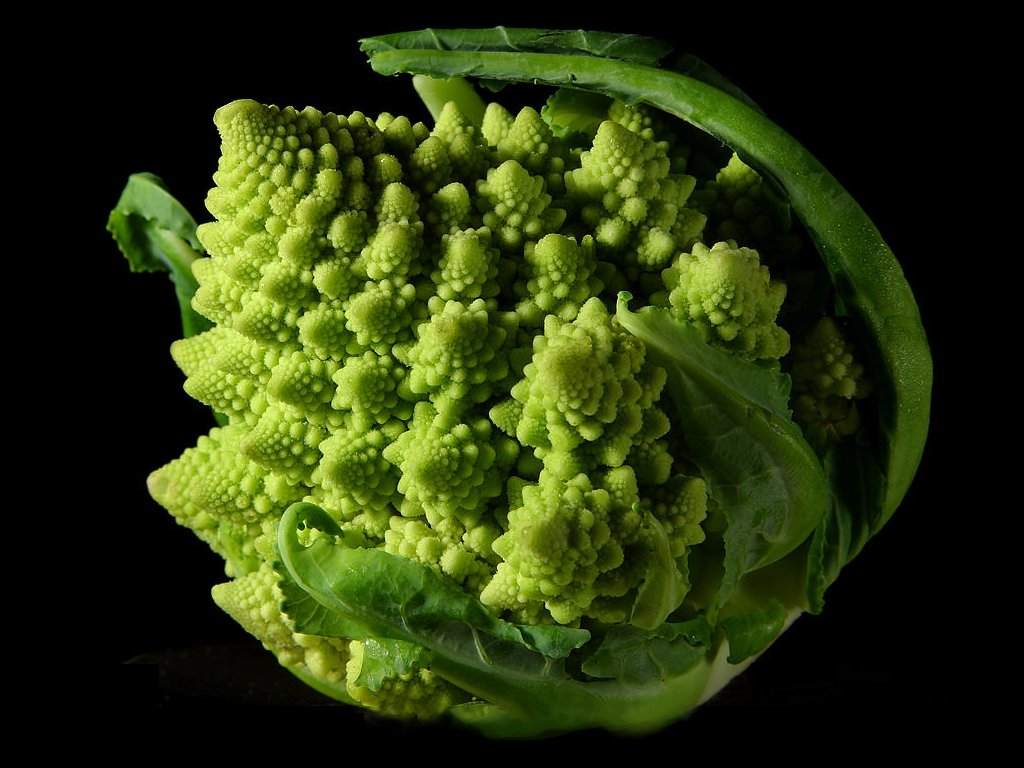
\includegraphics[width=7cm,height=7cm]{images/lettuce.jpg}
\end{center}
\end{frame}

\begin{frame}[fragile]
\begin{minted}{cucumber}
Feature: Compute factorial
    In order to play with Lettuce
    As beginners
    We'll implement factorial

    Scenario: Factorial of 0
        Given I have the number 0
        When I compute its factorial
        Then I see the number 1
\end{minted}
\end{frame}

\begin{frame}[fragile]
\begin{minted}{python}
from lettuce import *

@step('I have the number (\d+)')
def have_the_number(step, number):
    world.number = int(number)

@step('I compute its factorial')
def compute_its_factorial(step):
    world.number = factorial(world.number)

@step('I see the number (\d+)')
def check_number(step, expected):
    expected = int(expected)
    assert world.number == expected, \
        "Got %d" % world.number

def factorial(number):
    return -1
\end{minted}
\end{frame}

\begin{frame}
\begin{itemize}
\item Inspirováno {\bf Ruby} knihovnou {\tt Cucumber}
\item Test je popsán v čistém textu
\item Musí se definovat parsery jednotlivých kroků
\end{itemize}
\end{frame}


\section{Co dál?}
\begin{frame}
\begin{center}
\huge{Co dál?}
\end{center}
\end{frame}

\begin{frame}
\begin{itemize}[<+->]
\item {\bf Testy} automatizují ověřování, že kód funguje
\item Co potřebujeme teď, je {\bf automatické} spouštění testů.
\item {\bf Tox} -- testování v různých prostředích
\item {\bf CI} (Jenkins, Travis) -- spuštění testů při commitu do vcs
\item etc.
\end{itemize}
\end{frame}

\begin{frame}
\begin{center}
Děkuji za pozornost, trpělivost a všechny ty ryby.\\[2cm]

Otázky?

\vfill


tomas.ehrlich@gmail.com
\smallskip

Twitter: @tomas\_ehrlich
\end{center}
\end{frame}

\end{document}
